\documentclass{sig-alternate}

\title{Modern Techniques for Energy Optimization for Green Cloud Computing}

\author{
\alignauthor
 		David Donatucci\\
        Division of Science and Mathematics\\
        University of Minnesota, Morris\\
        Morris, MN 56267\\
        donat056@morris.umn.edu\\
}
\date{} 

\begin{document}
\conferenceinfo{UMM CSci Senior Seminar Conference, December 2014}{Morris, MN}
\pagestyle{plain}

\maketitle

\begin{abstract}

Place abstract here

\end{abstract}

\keywords{Cloud Computing, Green Computing}

\section{Introduction} \label{sec:intro}

Cloud Computing has been growing rapidly in the last several years in order to accommodate a growing demand for internet services. Due to this growth, larger data centers are required to meet demand. With larger data centers, an increasing amount power is necessary for these data centers to fulfill demands. In 2010, 1.5\% of all energy consumed worldwide was from data centers. In 2000, only about one fourth of that energy was used to power data centers~\cite{Yanggratoke}. In light of these staggering numbers, much research has been devoted to reducing power consumption. So far, two different approaches have been implemented to combat power consumption: macro-based and micro-based methods. Macro-based methods focus on exploiting data centers in diverse geographical locations that have higher levels of renewable energy or cooler climates. Micro-based methods focus on efficient resource allocation of data center components~\cite{Hassan}. A description of cloud computing, evolutionary algorithms, gossip-based protocol and the Hungarian method of assignment are provided in Section~\ref{Background}. Section~\ref{sec:MacAl} discusses a macro-based algorithm, and Section~\ref{sec:MicAl} provides details on mirco-based algorithms. The results of these algorithms are presented in Section~\ref{sec:results}, and ramifications of these algorithms are presented in Section~\ref{sec:conclusion}. Unfortunately, comparisons between these algorithms will not be discussed due to the fact that the algorithms were optimizing different parameters and there was not a standard representation of result data.
\pagebreak
\section{Background} 
\label{Background}

In order for the reader to fully understand the material presented in this paper, we will present some necessary background information.

\subsection{Cloud Computing}
\label{sec:Cloud Computing}

In the last several years, cloud computing has become a prevalent service. Cloud computing pertains to both the applications services provided via the Internet and the hardware and systems software in data centers. Inside these data centers are an exuberant amount of servers (the hardware) managed by middleware (software that communicates between servers). These components make up what is called the \emph{cloud}~\cite{Armbrust}. Usually, large IT firms called \emph{providers}, such as Google or Amazon, provide the hardware and system software for these large data centers. However, these large IT firms have extra servers and rent them to smaller companies providing a relatively cheap system to compute in the cloud. 

The workload on the cloud is amount of requests for service at a given time. A cloud is considered to be in \emph{overload} if there is not enough resources to handle all of the service requests. In order to provide a high quality of service, \emph{QoS}, the providers sign a service level agreement, \emph{SLA}, that requires them to fulfill these requests in a set amount of time. 

\subsection{Evolutionary Multi-objective Optimization Algorithms (EMOA)}
\label{sec:EMOA}

\begin{figure}[tb]
 \centering
 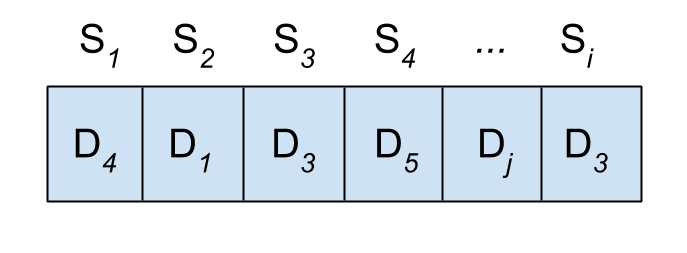
\includegraphics[height=0.15 \textwidth]{Individual}
 \caption{Example of a individual that is a potential solution to assigning cloud services, $S_i$, to data centers, $D_j$. Individuals, in this case, are stored as an array with the indices corresponding to a cloud service and the elements of the array corresponding to the data center in which that service is placed.}
 \label{fig:EMOA}
\end{figure}

Evolutionary Computation~\cite{poli08:fieldguide} is based around the interactions of \emph{individuals}. Individuals are similar to organisms in biological evolution but contain a solution to a given problem, see Figure~\ref{fig:EMOA}. As in biological evolution, a group of individuals makes up a population. In the process of biological evolution and natural selection, organisms within a population compete in order to survive and reproduce. Individuals best adapted to their environment have the best chance of fulfilling these objectives.  In an \emph{evolutionary multi-objective optimization algorithm}, EMOA, individuals also compete, but here those individuals that provide closer solutions to all user-defined optimizations have the best odds. The goal of EMOAs is to produce a set of individuals that provide quality solutions in a reasonable amount of time. 

At the beginning of an EMOA, a population is randomly initialized. The initial population then competes in order to be selected for alteration towards a better solution. For the purposes of this paper, we will discuss about binary tournament selection, although there are many different methods to select individuals to breed. Binary tournament selection is where two individuals are randomly chosen from the population, and the individual that is more optimized is selected as a parent. This is performed twice to obtain two parents.  These selected parents can propagate their genetic material to the next generation by two methods. The first and most common method is crossover, comparable to sexual reproduction, where two parents are selected from the current generation, and elements from each selected individual are combined to form a new individual in the next generation. The second method is mutation, in which an individual is selected and partial altered randomly, much like biological mutation. Crossover and mutation are utilized across multiple generations, until an optimized solution is found or until some sort of resource limit is reached. % need to explain what constitutes an individual in this case picture? and awkward working

\subsection{Gossip-based Protocol}
\label{sec:GBP}

\emph{Gossip-based}, GB, protocol acts exactly as the name gossip implies. A node which contains new information selects multiple nodes called \emph{peers} to spread new information to. The selection of peers is often probabilistic and therefore the number of peers is random. The act of spreading the information is called a \emph{round}. In the next round, each of the peers that received the information selects more peers to spread the information to. As more rounds are completed, all of the nodes eventually obtain the same new information~\cite{Yanggratoke}.

\subsection{Hungarian Method of Assignment}
\label{sec:HMA}

The following describes the general procedure of the Hungarian Method of Assignment. The \emph{Hungarian Method of Assignment} uses a $n \times n$ cost matrix with respect to energy in Figure~\ref{fig:HMA}. to find a solution for the minimum configuration of server to job placement where rows and columns represent jobs and servers respectively~\cite{Han}. The matrix elements represent the amount of power placing a job onto a server. To find this configuration, we first subtract the smallest wattage in each row from all the entries of its row. Similarly, we subtract the smallest wattage (after rows have been subtracted) in each column from all entries in its column. After subtraction, the new cost matrix will have some number of zero entries. Since we only subtract the minimum entries,there will not be any negative entries. Draw lines through appropriate rows and columns so that all the zero entries of the cost matrix are covered and the minimum number of such lines is used.  If the number of lines is equal to n then there is an optimal solution. However, if the number of line is not equal, then we determine the smallest entry not covered by any line. Subtract this entry from each uncovered row, and then add it to each covered column repeating until there are n lines.  We then can easily determine the the optimal solution. 

\begin{figure}[tb]
 \centering
 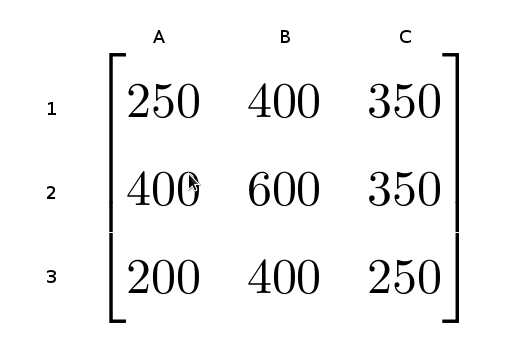
\includegraphics[height=0.25 \textwidth]{s}
 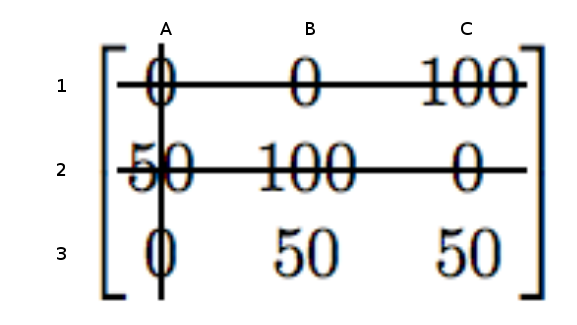
\includegraphics[height=0.20 \textwidth]{s2}
 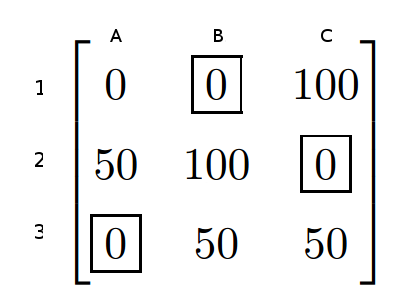
\includegraphics[height=0.25 \textwidth]{s3}
 \caption{Computing the Hungarian method cost matrix for servers A,B,C and jobs 1,2,3. Numbers are represented in Watts. The optimal solution (job to server) is 1-B, 2-C, 3-A}
 \label{fig:HMA}
\end{figure}

\section{Macro-based Algorithms}
\label{sec:MacAl}

\emph{Green Monster} is an framework proposed by Phan et al that uses geographical location to maximize energy savings by mainly emphasizing the maximization of renewable energy. The EMOA, described in Section~\ref{sec:EMOA}, in Green Monster uses three optimization objectives: renewable energy consumption (RE), cooling energy consumption (CE), and user-to-service distance (USD). In order to get the best results, Green Monster looks to maximize RE, and minimize both CE and USD. By minimizing the USD, Green Monster attempts to minimize the response time to assure a high quality of service specified by the SLAs. Also, minimizing the CE implies that the energy consumed in the data center will be more heavily used for processing. In \ref{sec:GMEMOA}, we will discuss how the EMOA behind Green Monster works, and in \ref{sec:GMSims} we will look at simulations of Green Monster with real world data.~\cite{Phan}

\subsection{Green Monster EMOA}
\label{sec:GMEMOA}

Green Monster represents individuals an a configuration of all services (S$_{\text{\emph{i}}}$) in all data centers (D$_{\text{\emph{j}}}$). Each data center has a service capacity
%(C$_{\text{\emph{i}}}$) !!could put equations in for RE CE USD!! ~\ref{sec:EMOA} where to put?
or the maximum workload a data center can handle. To initialize a population of \emph{N} individuals, the EMOA assigns random services to random data centers so that any given data center does not exceed the service capacity. If the service does exceed the service capacity, it will be assigned to the data center with the least workload. Upon completion, the EMOA uses binary tournament selection to select individuals for alteration. In this instance of binary tournament, the individual is selected by~\emph{constrained-dominance}. An individual, \emph{i},  is constrained-dominant to an individual, \emph{j}, if \emph{i} has the least amount of service capacity violations or if \emph{i} and \emph{j} do not have any violations \emph{i} is automatically constrained-dominant. When two parents are selected, crossover is performed determined by a crossover rate and two offspring are produced. Both of these offspring perform mutation determined by a mutation rate for each service. Mutating simply switches the current data center, D$_{\text{\emph{j}}}$, for a random new one.

Phan et al then perform a local search based on a local search rate
%should i put 10%
for each S$_{\text{\emph{i}}}$. This local search checks to see if any D$_{\text{\emph{k}}}$ where ${\text{\emph{k} ${\neq}$ j}}$, could improve all optimizations without violating the service capacity. If D$_{\text{\emph{k}}}$ meets the previous criteria, then D$_{\text{\emph{k}}}$ replaces D$_{\text{\emph{j}}}$ in S$_{\text{\emph{i}}}$. This is done repeatedly until the same amount of individuals in the parent generation are in the next generation. In order for the best individuals to permeate to the next generation, Phan et al combine both the parent and offspring generations and sort them based on constrained-dominance. Phan et al then take only the first \emph{N} individuals. This whole process repeats until a certain number of generations is reached. 

\subsection{Green Monster Simulations}
\label{sec:GMSims}
 
Several simulations of Green Monster have been conducted based on statistics of nine data center in nine different European countries: Denmark, Germany, Greece, Ireland, Italy, Netherlands, Spain, UK and Portugal. Temperature data was used from European Climate Assessment \& Dataset project which records real temperature data in Europe. These countries were chosen based on the wide variety of climates and renewable energy. The average renewable energy production data was pulled from each country from January 2007 to December 2009. In each data center there are between 8-200 servers and 16-400 services consisting of voice, data, and video based on the countries population. For the simulation, Phan et al decided that every server will have the same specifications and each type of service was evenly distributed to all types of services. Data center configurations are given in Table~\ref{tab:DCConfig}.  Green Monsters EMOA in this simulation runs bi-weekly for twelve months. After running the EMOA with the configurations in Table~\ref{tab:EMOAConfig}, the individual that is the most optimized overall is selected. Green Monster will migrate service, S$_{\text{\emph{i}}}$, to data center, D$_{\text{\emph{j}}}$, according to solution presented by the optimized individual.

\begin{table}[tb]
\begin{center}
\begin{tabular}{|l|l|}
    \hline
    \multicolumn{2}{|c|}{\textbf{Data Center Configurations}} \\
    \hline
    Number of Data Centers & 9 \\
    Total Number of Servers In Data Centers (\emph{N}) & 100 \\
    Service Types & 3 \\
    Average rate of requests per day & 2,000,000 \\
    Max Power Consumption in a Server & 400W \\
   	Min Power Consumption in a Server & 150W\\
    \hline
\end{tabular}
\caption{Data center configurations in Green Monster simulation}
\label{tab:DCConfig}
\end{center}
\end{table}

\begin{table}[tb]
\begin{center}
\begin{tabular}{|l|l|}
    \hline
    \multicolumn{2}{|c|}{\textbf{EMOA Configuration}} \\
    \hline
    Generations & 100 \\
    Population size (\emph{N}) & 100 \\
    Crossover rate & 90\% \\
    Mutation rate & 10\% \\
    Local Search rate & 10\% \\
    \hline
\end{tabular}
\caption{EMOA configurations in Green Monster. Configurations were based on optimal experimental results by Phan et al.}
\label{tab:EMOAConfig}
\end{center}
\end{table}



\section{Micro-based Algorithms} 
\label{sec:MicAl}

There are many different micro-based algorithms for a green cloud, but we will choose to focus on two algorithms underdevelopment: GRMP-Q, a gossip-based allocation algorithm and the speed-scaling algorithm by Yanggratoke et al. 
\subsection{Gossip-based Resource Allocation}
\label{sec:GBRA}

%The first section is divided into two sections to describe the basics of GRMP-Q,~\ref{subsec:GRMPBasics}, and the second section~\ref{sub:GRMPSim} describes GRMP-Q in simulations. 
%\subsubsection{GRMP-Q Basics}
%\label{subsec:GRMPBasics}

\emph{GRMP-Q} is middleware for a data center that utilizes gossip protocol, described in Section~\ref{sec:GBP}, to minimize the amount of servers running services. Usually, providers rent specific servers by the hour to smaller companies. This, however, is not efficient. A single server working at  \emph{workload capacity}, or the maximum amount of services that a single server can handle, will be much more efficient than three servers working at one third of workload capacity. This is due to the minimum power level that a server must consume to be on. GRMP-Q attempts to migrate all services to the least number of servers possible.  For simplicity, Yanggratoke et al assume that all servers, \emph{N}, in a data center have identical specifications (power consumption, CPU, and memory capacities). For any given service, ($S_i$), the demand, \emph{$\omega_{S_i}$}, can be spread across multiple servers. The equation for demand $\omega_{(S_i,n)}$ on a single server \emph{n}, is given by \eqref{eq:1} where $\alpha_{(S_{i},n)}$ is a portion of the demand of $S_{i}$ running on server \emph{n}:
\begin{equation}
\omega(S_{i},n) = \alpha_{(S_{i},n)} \omega_{S_i} \text{\emph{~such that~}} \alpha_{(S_{i},n)} \geq 0,~ \sum_{n=1}^{N} \alpha_{(S_{i},n)} = 1 \label{eq:1}
\end{equation}

Yanggratoke et al then placed all of the \emph{$\alpha_{(S_{i},n)}$} for every service into a matrix called \emph{the configuration matrix}. The configuration matrix, A, shows how the data center's resources are allocated to services. At certain times, load changes, addition of services, or change in the number of servers will cause the configuration matrix to be updated. 

The first objective of GRMP-Q is to satisfy user demand by allocating enough resources so that the provider can satisfy the SLA. The second objective is to minimize power consumption. GRMP-Q does this by turning a server to stand-by if the total demand on the server is zero. If there is insufficient resources or the \emph{$\omega_{(S_{i+1},n)}$} of a new service, S$_{\text{\emph{(i+1)}}}$, is greater than the workload capacity, $\Omega$, the system will turn a stand-by server on. 

In order to transfer one service to another service there are three gossip-based processes that occur. The first process is initialization which initializes the gossip protocol for the current configuration matrix at a random server \emph{n}.  The second process chooses a peer from the configuration matrix by randomly selecting a different server, \emph{j}, with $\alpha > 0$. After a peer is selected, the relative demand, \emph{y}, on server \emph{n} is calculated by taking the sum of \emph{$\omega$} of all services on \emph{n} divided by the workload capacity of \emph{n} shown in~\eqref{eq:2}.
\begin{equation}
y_n = \sum_{i=1}^M \omega_{(S_i,n)}/\Omega \textit{~where M is the total num of services}\label{eq:2}
\end{equation}

If $y_n + y_j \geq 2$, the algorithm assumes based on these two servers that the cloud is in overload and will move services to the server that has a smaller relative demand. However, if $y_n + y_j < 2$, then algorithm assumes the cloud is in \emph{underload} (there are unused resources on some active servers). When the cloud is in underload, GRMP-Q then packs services in such a manner that the server with the highest relative demand of $y_n$ and $y_j$ migrates services so that demand is equal to $\Omega$. This ensures that one server is fully packed and the other is less than $\Omega$. Since this algorithm is gossip-based,  comparisons of two servers will occur continuously~\cite{Yanggratoke}.  
%to add memory, maybe simulation?

%\subsubsection{GRMP-Q Simulations}
%\label{sub:GRMPSim}


\subsection{Speed-Scaling}
\label{sec:Speed}
In this version of speed scaling, Han et al use a combination of performance optimization and job placement to make data centers more energy efficient. Han et al define the power consumption with respect to CPU speed, \emph{s}, given by \eqref{eq:3}. 
\begin{equation}
P_{i,j} = s_{i,j}^{\gamma}+ c \textit{~where j is a specific job and i is the server number}\label{eq:3}
\end{equation}
\begin{equation}
W_{i} =\sum_{j=1}^J \lambda_{j} \times P_{i,j}\textit{~where J is the total number of jobs}\label{eq:4}
\end{equation}
\begin{equation}
U =\sum_{i=1}^M W_{i} \textit{~where M is the total number of servers}\label{eq:5}
\end{equation}

where $c$ accounts for static power loss and $\gamma$ is some constant that was computed experimentally. Han et al found $\gamma \approx 3$ for the relationship between speed and power. In order to relate jobs and the QoS, jobs have a weighted positive integer $\lambda_j$ that denotes the level of QoS for job \emph{j}. The total weighted power for a server is shown in \eqref{eq:4} such that \emph{j} is the total number of jobs on the server. The total weighted power, U, is given by \eqref{eq:5} where \emph{M} is the total number of servers in the data center.

Han et al assume for this algorithm that there are \emph{j} jobs and \emph{M} servers. Han et al then adopt an implementation of the Hungarian method of assignment described in Section~\ref{sec:HMA}, to assign jobs to servers. Han et al then hypothetically migrate the jobs to the appropriate servers, adjusts the speeds of CPUs such that there is no extra processing power utilized, and then recomputes U. If the $\Delta U \geq 0$ then the algorithm will actually migrate the jobs to the appropriate servers~\cite{Han}. 

\section{Results} 
\label{sec:results}

The results of the three different algorithms are discussed in this section.

\subsection{Green Monster}
\label{sec:GM}
\begin{table}[tb]
\begin{center}
\begin{tabular}{|l|l|l|l|}
    \hline
    \multicolumn{4}{|c|}{\textbf{Daily Averaged Objective Values for Green Monster}} \\
    \hline
    & RE &  CE & USD \\
    \hline
    Static (\emph{N}) & 324.5 & 949.58 & 0 \\
    Random rate & 327.3 & 947.34 & 487378\\
   	Green Monster & 438.5 & 919.02 & 373172\\
    \hline
\end{tabular}
\caption{Daily averaged objective values for static placement, random placement, and Green Monster. RE and CE are in MWH. }
\label{tab:GMV}
\end{center}
\end{table}

Phan et al simulated their algorithm in comparison to two benchmark algorithms, static placement policy and a random placement policy. Static placement randomly selects two services and places them on each server for the duration of the simulation. Random placement dynamically migrates biweekly by using the random initial population generation described in Section~\ref{sec:GMEMOA}. According to the results in Table~\ref{tab:GMV}, Green Monster consumed a significantly higher amount of renewable energy than either static or random. The daily average of RE utilized by Green Monster was 111 MWH, or 33.9\%, more than either algorithm. This shows that Green Monster migrates services to more renewable data centers.  Table~\ref{tab:GMV} also illustrated that Green Monster saves more cooling energy than the other algorithms. Green Monster saves 3.2\% more cooling energy than the random placement algorithm on a daily average basis. However, the main focus was to maximize renewable energy. Green Monster also surpassed random placement yielding a 23.4\% shorter USD than random.  Notice that static placement has a USD of zero. This is because the static placement does not migrate any service during the twelve months~\cite{Phan}.   


\subsection{GRMP-Q}
\label{sec:GRMP-Q}

GRMP-Q was simulated on a data center with 10,000 servers in order to analyze the reduction of power. Yanggratoke et al implemented several different loads on the cloud: 10\%, 40\%, 70\%, 100\%, 130\% of the CPU resources in the cloud shown in Figure~\ref{fig:Results_PR}. When the load on the cloud was small, 10\%, the reduction of power increased by 85\% from a cloud in which none of the servers switch to stand-by. As expected, power reduction becomes smaller but still saves around 15\% of power at a cloud load of 70\%.  However, this algorithm does not provides any benefit from an overloaded cloud.  In order to test if this algorithm was scalable, Yanggratoke et al ran simulations for a cloud with as little as 2,500 servers to as many as 160,000 servers evaluated at a cloud load of 25\% and 50\%. In all cases, Yanggratoke et al found that the amount of servers does not affect the amount of power reduction. Power reductions were around 25\% and 60\% for a cloud load of 25\% and 50\% respectively~\cite{Yanggratoke}.  

%add scalablitity graph not exciting.

\begin{figure}[tb]
 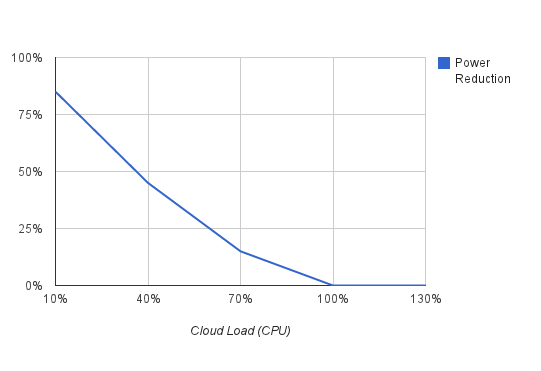
\includegraphics[height=0.35 \textwidth]{image}
 \caption{Power reduction of GRMP-Q with respect to cloud load. }
 \label{fig:Results_PR}
\end{figure}

\subsection{Speed Scaling}
\label{sec:SS}

Han et al simulate their algorithm in comparison with a non-power aware policy and a dynamic voltage and frequency scaling, \emph{DVFS}, policy. In a non-power aware (\emph{NPA}) system, there are no optimizations regarding placement of jobs. In a DVFS, all servers are set to proportional speeds by estimating the CPU speed required for its current running jobs. DVFS will also adjust the voltage which means that circuits in the processor will switch more slowly with a lower voltage. In Figure~\ref{fig:Results_SS},  we can clearly see results indicate that the proposed algorithm uses significantly less energy per hour than either NPA or DVFS policies~\cite{Han}.

%scalability? from figure

\begin{figure}[tb]
 \centering
 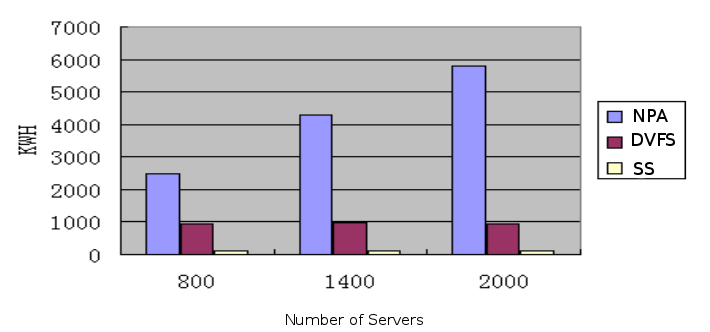
\includegraphics[height=0.2 \textwidth]{s4}
 \caption{Number of servers with respect to power in kilowatt hours. Non-power aware (\emph{NPA}). Dynamic Voltage and Frequency Scaling (\emph{DVFS}). Han et al's algorithm (\emph{SS}).}
 \label{fig:Results_SS}
\end{figure}

\section{Conclusions} 
\label{sec:conclusion}

From the results, we can tell that both micro-based and macro-based algorithms produce a greener data center even though they use completely distinct methods to do so.  Green Monster focuses on migrating services to different data centers so that more renewable energy is conserved. GRMP-Q targets the packing of services into in minimum amount of servers possible. Han et al centers around adjusting CPU frequency and voltage while optimizing the placement of jobs on servers. Since cloud computing is still relatively new and growing, there is considerable potential to reduce power even further. Combinations of both micro and macro will undoubtedly be used together to reduce power consumption of data centers.

\section*{Acknowledgements}

Many thanks to my advisor, Elena Machkasova, and somebody else for being my second reader. 


\pagebreak
\bibliographystyle{acm}
\bibliography{annotated_bibliography}

\end{document}